\NeedRoom{10}

\subsection{Speed, Sensitivity, and Inventory Boundary}

\begin{figure}[htbp]\centering

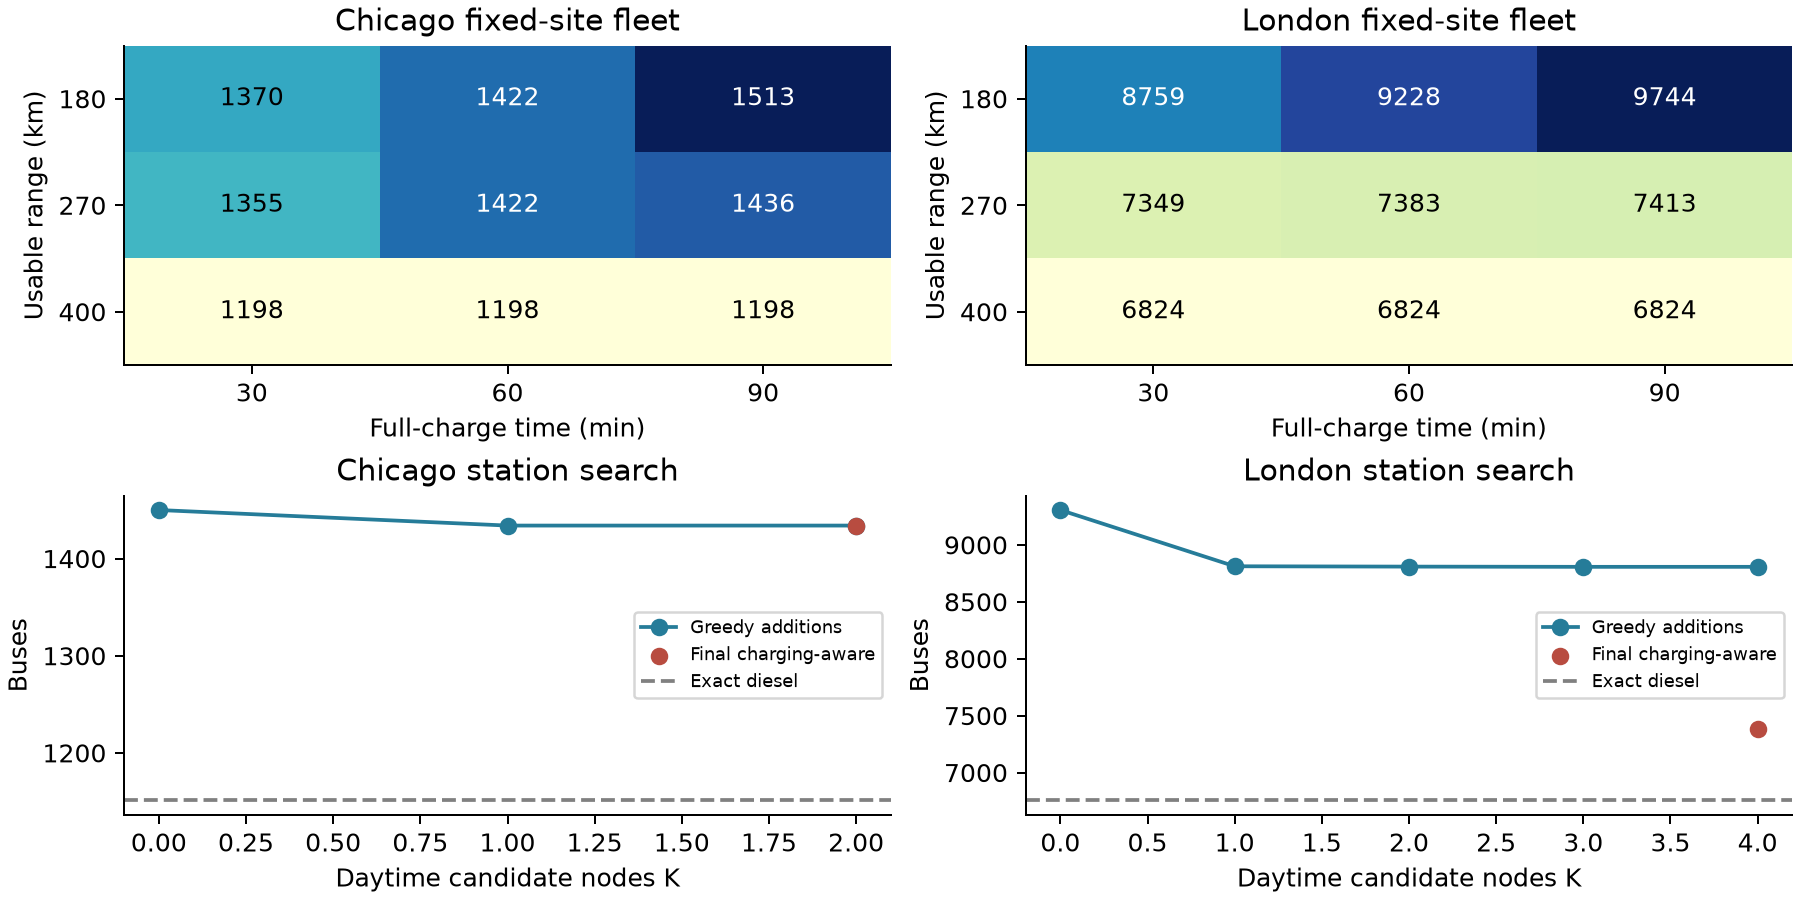
\includegraphics[width=\textwidth,height=0.37\textheight,keepaspectratio]{images/comparator_sensitivity.png}

\caption{Fixed-site feasible upper bounds by range and charge time (top), plus greedy station traces and charging-aware final solutions (bottom). Raw heuristic counts remain in JSON.}\label{fig:result6}

\end{figure}

\begin{longtable}{@{}L{\dimexpr 0.39000\textwidth-2\tabcolsep\relax}L{\dimexpr 0.30500\textwidth-2\tabcolsep\relax}L{\dimexpr 0.30500\textwidth-2\tabcolsep\relax}@{}}
\caption{Separate inventory-cohort renewal comparison}\label{tab:source16}\\
\toprule
\textbf{Inventory-renewal comparison} & \textbf{Chicago} & \textbf{London} \\
\midrule
\endfirsthead
\multicolumn{3}{l}{Table \thetable\ (continued)}\\
\toprule
\textbf{Inventory-renewal comparison} & \textbf{Chicago} & \textbf{London} \\
\midrule
\endhead
\midrule\multicolumn{3}{r}{Continued on next page}\\\endfoot
\bottomrule\endlastfoot
Inventory scope & 1,875 at year end & 8,643 at 31 March 2023 \\
Initial electric evidence & 25, inferred June state & 950 observed in audit \\
Life cap tested here & 17 years & 17 years \\
Minimum peak annual renewal & 539 & 776 \\
Total renewed positions & 1852 & 7759 \\
\end{longtable}

The original cohort optimizers are also re-executed; London includes 12- and 14-year life sensitivities. Fleet stock contains reserves and existing technologies, whereas timetable counts are active homogeneous vehicles. London geographic bus coverage also differs from its TfL contract inventory. The two outputs must not be merged into an unsupported purchase total.


Different route lengths, operating windows and endpoint geometry change the route scores and charging opportunities. Actual local costs and route-assigned ages could reverse the illustrated order. Four candidate nodes, or even a smaller selected set, do not establish physical charging sufficiency.

